% ======================================================================
% QUICK DRAFT — in silico / computational article
% Microwave reheating of e-beam-pumped rare-gas-halide laser plasmas
%
% !! BEFORE ANY CIRCULATION OUTSIDE THE GROUP !!
%   * EXPORT-CONTROL / DATA-RIGHTS REVIEW REQUIRED. Some operating
%     parameters trace to a program document marked export-controlled /
%     data-rights (see docs/DE-AR_targets.txt header). Every such number
%     is used here as a modeling choice; the award document is neither
%     quoted nor cited. Review before submission anyway.
%   * Funding/acknowledgment text intentionally left as a placeholder —
%     insert the program-approved statement verbatim; never paraphrase.
%   * Citations marked [verify] are placeholders — complete them.
%
% Build: pdflatex mw_reheat_draft.tex  (twice; figures from make_figs.py)
% All numbers are read from recorded run artifacts:
%   SPECK/rebuild_out/mw_benchmarks/{mw_benchmarks_loki,ib_feasibility,
%     afterglow_nogo_audit{,_arf},sign_decidability}.json
%   SPECK/rebuild_out/copump_scan/copump_verify.json
%   SPECKLE/runs/*.json
% and the REBUILD CHANGELOG entries [0.1.20]-[0.1.28].
% ======================================================================
\documentclass[aps,pra,preprint,longbibliography,nofootinbib]{revtex4-2}

\usepackage{graphicx}
\usepackage{amsmath}
\usepackage{xcolor}
\newcommand{\todo}[1]{\textcolor{red}{[TODO: #1]}}

\begin{document}

\title{Microwave reheating of electron-beam-pumped rare-gas--halide
laser plasmas:\\ a robust observable, a real but marginal channel}

\author{Cooper K.\ Watson}
\affiliation{Texas A\&M University\todo{verify department/affiliation line}}

\date{\today}

\begin{abstract}
Whether microwave energy added to an electron-beam-pumped KrF/ArF laser
plasma can improve its performance is assessed \emph{in silico} across
three independently constructed electron treatments: a 26-species
zero-dimensional kinetics engine with interchangeable electron-rate
tiers (LoKI-MC swarm tables and rates measured by an in-house PIC/MCC
code), and an independently developed one-dimensional discharge-pumped
fluid model with an in-tree two-term Boltzmann solver. Using twin-pair
numerical experiments (identical runs with and without a
prescribed-power microwave window) over eight benchmark configurations,
we find a three-part answer. (i)~Reheating is a \emph{robust
observable}: the gain-proportional sidelight fluorescence rises in
every benchmark on both rate tiers and in the independent model
($+1.5\%$ to $+12\%$), so hybrid-pumping experiments that monitor
fluorescence will genuinely detect the microwave. (ii)~One
laser-energy-positive channel is \emph{real and is not an artifact}:
afterglow reheating of a high-optical-margin cell that is still
extracting raises laser output by ${\sim}+10\%$ per microwave joule,
and this sign survives all 41 rate-uncertainty and literature-conflict
bracket variants ($+8.3\%$ to $+12.9\%$) and a change of electron-rate
tier in a sibling configuration --- and it is reproduced at the same
${\sim}+10\%$ scale in the independent one-dimensional model, where
its predicted margin, window-timing, and deposition-locality
dependences are verified ladder by ladder under timestep refinement.
(iii)~Exploiting it is \emph{very difficult}: at a
program-representative coupling budget (250~kW per litre) no benchmark
changes its blended intrinsic efficiency by more than
$0.006$~percentage points; the conductive plasma pins the settled
reduced field at ${\lesssim}2$~Td at any injected power, both excimer
supply chains weaken when the electrons are heated, the wall-plug
inequality $\eta_{\rm source}\times m>\eta_{\rm beam}\approx7\%$ is
barely reachable even by magnetron-class sources, and the sign of the
during-pulse variant is hostage to a single rate coefficient (positive
only if $e+\mathrm{Kr}^*\!\to\mathrm{Kr}^++2e$ lies within a factor
$\times0.49$--$\times1.99$ of its nominal value). We state what would
decide each remaining open question: a factor-two determination of
that one rate, and gain-referenced twin-shot experiments whose
absorbed-energy denominator is closed by a full-wave deposition map.
\end{abstract}

\maketitle

\section{Introduction}

Electron-beam-pumped rare-gas--halide lasers (KrF at 248.5~nm, ArF at
193~nm) remain the leading broadband-ultraviolet driver candidates for
inertial fusion energy, and their intrinsic efficiency --- of order
7--10\,\% in the best demonstrated devices
\cite{electra}\todo{verify} --- is the quantity every driver study
tries to raise. A recurring proposal is \emph{hybrid pumping}: keep the
electron beam as the primary ionizer and add electromagnetic power
(microwave-band, waveguide-coupled) to reheat the electron population,
either during the pump pulse or in the recombining afterglow, in the
hope of harvesting additional excimer formation from the ion--ion and
harpoon chains \cite{hybridconcept}\todo{verify or drop}.

The proposal is attractive because the microwave subsystem is cheap
relative to the beam, and because experiments monitor a convenient
surrogate: the sidelight fluorescence at the lasing wavelength, which
is proportional to the small-signal gain. It is also easy to test badly
--- a fluorescence increase does not by itself demonstrate an
efficiency increase, and a simulated efficiency increase can be an
artifact of a single uncertain rate coefficient, of a solver tolerance,
or of a timestep. This article is a falsification-first computational
study designed to separate those outcomes. We ask three sharply
distinguishable questions: Is reheating \emph{observable}? Is any
laser-energy gain \emph{real} in the sense of surviving every
model-side perturbation we can apply? And what does it \emph{cost} to
exploit?

Our contribution is methodological as much as physical. Every claimed
sign is subjected to a decidability ladder --- solver and integrator
convergence, an exchange of the complete electron-rate tier between
independently produced sets, brackets of $\times\tfrac13..\times3$ on
every estimated rate plus literature-conflict alternates, and
replication in an independently written model of a different pumping
geometry --- and any sign that fails a rung is reported as
\emph{undecided}, together with the measurement that would decide it.

\section{Models and methods}

\subsection{Three electron treatments}

\emph{(a) Zero-dimensional kinetics engine (``REBUILD'').} A 26-species
KrF/ArF plasma-chemistry engine (electrons, electron energy, gas
temperature, cavity photon field, and a closed four-channel energy
ledger integrated as state) with ${\sim}169$ reactions in the KrF
configuration. Beam deposition uses Spencer--Fano-partitioned yields;
the laser field is a mean-field cavity with an intracavity absorber
inventory. The engine is predictive-only: literature anchors are scored
against, never fitted to. Two interchangeable electron-rate tiers
supply every electron-impact rate: (i)~a \textsc{LoKI-MC} swarm-table
tier \cite{loki}\todo{verify LoKI-MC citation} keyed by mean electron
energy, with measured relaxation-bridged curves below table coverage,
and (ii)~a \emph{kinetic} tier of rates measured by an in-house 3-D
PIC/MCC code from the same cross-section sets. Agreement between tiers
is diagnostic, not enforced.

\emph{(b) PIC/MCC rate source.} The kinetic tier's rates are exported
from particle simulations (Monte Carlo collisions on the full
cross-section set) as rate-versus-mean-energy curves; they share
nothing with the swarm tier but the cross sections.

\emph{(c) Independent 1-D discharge model.} A one-dimensional
charged-fluid model of a discharge-pumped KrF laser
(Scharfetter--Gummel transport, Poisson field, magnetic-pulse-
compression circuit, 45-channel reduced kinetics, in-tree two-term
Boltzmann solver refreshed from the local mean energy), developed
independently by another author \cite{oned}\todo{citation/permission
for the 1-D model}. We drive it unmodified through a subclass that adds
a bounded prescribed-power heating term at the model's own
deliverable-heating seam; the microwave energy is metered externally.

\subsection{Twin-pair experiments and metrics}

Every reheat question is posed as a \emph{twin pair}: two runs
identical in every input except that one carries a trapezoidal
microwave window of prescribed \emph{injected power} $P_{\rm MW}$
(power, not field: a prescribed field across a conducting plasma is an
unbounded generator --- in an early design study a held 8~Td window
drove a cell to full ionization while the energy ledger closed
perfectly; the bookkeeping was right and the model assumption wrong).
In the 0-D engine the field settles each step at the lowest reduced
field $E/N$ at which the swarm absorption
$e\,n_e\,v_d(E/N)\,E\,\nu^2/(\nu^2+\omega^2)$ matches the prescribed
power, capped at 30~Td. Windows: \emph{afterglow} (opening 10~ns after
beam end, 150~ns flat) and \emph{co-pump} (the second half of the beam
pulse). The coupling budget follows a program-representative rule of
250~kW per litre of pumped volume at 95~GHz (the one X-band
configuration retains its own hardware value).

Metrics: the \emph{marginal} $m=\Delta E_L/E_{\rm MW}$ (laser energy
gained per microwave joule delivered); the \emph{blended} intrinsic
efficiency $\eta=E_L/(E_{\rm beam}+E_{\rm MW})$, whose change
$\Delta\eta$ answers the efficiency question with the microwave in the
denominator; and the post-beam fluorescence energy
$E_{\rm fl}=\int (n_{B}/\tau_{B})\,h\nu\,V\,dt$ over the window, the
experimental observable.

\subsection{The decidability ladder}

A sign is reported as \emph{decided} only if it is invariant under:
(1)~numerics --- seven solver settings including an independent
integrator (twin differences agree to $z\approx3.7\times10^3$ in the
reference case); (2)~the electron-rate tier swap; (3)~brackets of
$\times\tfrac13$ and $\times3$ on every estimated-provenance rate and
every literature-conflict alternate, applied to both twins; and
(4)~where expressible, replication in the independent 1-D model,
including timestep refinement. Anything else is \emph{undecided}, and
we compute what would decide it.

\section{Results}

\subsection{Reheating is a robust observable}
\label{sec:observable}

Table~\ref{tab:bench} collects the eight benchmark configurations: two
program-class cells that are sub-threshold in this engine, the
program's high-power cell, an X-band-equipped chamber column, two
optimized operating points found by a lever scan (Ar- and Ne-buffered),
and two literature anchor cells (a 1985 KrF kinetics benchmark and a
large ArF device at its recorded peak-efficiency point)
\cite{kannari,electra}\todo{verify}.

The post-beam fluorescence rises with the microwave on in \emph{all
eight} cases, on both rate tiers, spanning $+0.07$ to $+15$~mJ over the
window at the stated coupling rule. The independent 1-D model agrees:
at its lasing point the afterglow window raises its fluorescence proxy
by $+11.8\%$. This is the answer to the observability question, and it
carries a warning for experiment design: a hybrid-pumping campaign that
scores the microwave by gain-proportional fluorescence will see a
positive response \emph{even in configurations where the laser output
falls} (six of eight afterglow cases in Table~\ref{tab:bench}). The
fluorescence statement and the efficiency statement are different
statements.

\begin{table*}[t]
\caption{\label{tab:bench}Twin-pair results across the benchmark set
(swarm tier, corrected engine; coupling rule 250~kW/litre). Marginal
$m=\Delta E_L/E_{\rm MW}$; $\Delta\eta$ is the blended-efficiency
change in percentage points (microwave joules in the denominator);
$\Delta E_{\rm fl}$ is the post-beam fluorescence change for the
afterglow window. The two sub-threshold cells lase in neither twin.}
\begin{ruledtabular}
\begin{tabular}{lcccccc}
 & & \multicolumn{3}{c}{afterglow window} &
 \multicolumn{2}{c}{co-pump window} \\
case & $\eta_0$ (\%) & $m$ (\%) & $\Delta\eta$ (pp) &
 $\Delta E_{\rm fl}$ (mJ) & $m$ (\%) & $\Delta\eta$ (pp) \\
\hline
program class, 3 atm (Ar)   & no lasing & --- & --- & $+0.07$ & --- & --- \\
program class, 3 atm (Ne)   & no lasing & --- & --- & $+0.18$ & --- & --- \\
high-power cell, 2 atm      & 1.54 & $-2.8$  & $-0.0055$ & $+0.48$ & $+12.5$ & $+0.0029$ \\
X-band chamber column       & 2.16 & $-10.4$ & $-0.0036$ & $+2.15$ & $-1.9$  & $-0.0004$ \\
Ar-optimized point          & 4.95 & $-2.1$  & $-0.0056$ & $+5.12$ & $+1.3$  & $-0.0010$ \\
Ne-optimized point          & 6.19 & $\mathbf{+10.0}$ & $\mathbf{+0.0024}$ & $+1.30$ & $+5.1$ & $-0.0002$ \\
KrF anchor cell (1985)      & 0.70 & $-0.0$  & $-0.0003$ & $+0.47$ & $+3.0$  & $+0.0002$ \\
ArF anchor, 1.09 atm        & 6.13 & $-1.3$  & $-0.0031$ & $+14.8$ & $+5.7$  & $-0.0001$ \\
\end{tabular}
\end{ruledtabular}
\end{table*}

\subsection{One laser-positive channel is real --- and it is not an
artifact}
\label{sec:real}

Exactly one benchmark gains laser energy from afterglow reheating: the
Ne-buffered optimized cell, whose marginal is $+10.0\%$
($\Delta\eta=+0.0024$~pp). Three independent tests argue this is
physics, not numerics or a rate accident.

\emph{Bracket robustness.} Re-running the twin pair under every
estimated-rate bracket ($\times\tfrac13$ and $\times3$) and every
literature-conflict alternate --- 41 variants --- leaves the marginal
positive in \emph{all 41}, spanning $+8.3\%$ to $+12.9\%$
[Fig.~\ref{fig:robust}(a)]. Notably, the rate that controls the
co-pump sign (Sec.~\ref{sec:difficult}) moves this marginal by less
than one percentage point.

\emph{Cross-tier and cross-model witnesses.} The same
high-margin-afterglow class appears on the independent kinetic rate
tier in the sibling Ar-optimized cell ($-2.1\%$ on the swarm tier,
$+9.5\%$ kinetic), and in the independent 1-D discharge model, whose
afterglow marginal $+0.89\%\to+1.06\%$ is stable under timestep
halving. No single case is yet confirmed positive on \emph{both} tiers
--- the Ne-optimized kinetic-tier run is computationally severe and
still integrating --- so we state the class-level claim only.

\emph{Mechanism.} A row-flux audit of every excimer-formation channel
shows why this case is special and the others are not: all direct
formation rows are heavy-particle, and heating the electrons
\emph{weakens both supply lines} (the F$^-$ fuel of the ion--ion rows
via attachment, $\times0.13$ from 0.5 to 3~eV; the metastable fuel of
the harpoon rows via dissociative-recombination throughput,
$\times0.37$). The gain in the one positive case is not afterglow
harvest at all --- it is \emph{late extraction}: the high-margin cavity
is still draining while the window runs
($\Delta E_L \gg \Delta E_{\rm fl}$ there), i.e.\ a late co-pump of a
still-lasing cell. The channel is real, small, and conditional on
optical margin.

\emph{One-dimensional verification.} If the gain is late extraction,
three predictions follow: it must grow with the optical margin, die as
the window slides past the cavity drain, and depend on \emph{when} far
more than on \emph{where} the power is deposited across the gap. All
three hold in the independent 1-D model [Fig.~\ref{fig:oned}].
Scanning the output coupler at fixed drive, the marginal rises
monotonically ($+0.01\%$, $+0.20\%$, $+0.78\%$, $+0.9\%$ for
$r_{\rm out}=0.3$--$0.9$) even though the \emph{absolute} laser output
peaks at $r_{\rm out}=0.6$: the marginal follows the photon lifetime
--- the drain-overlap knob --- not the laser performance. At the
high-margin point, extending the integration horizon to capture the
full drain raises the marginal to $+5.7\%$ ($+10.1\%$ at half
timestep; robustly positive, magnitude unconverged upward) ---
quantitatively the same ${\sim}+10\%$ class as the 0-D channel.
Sliding the same window later collapses it: $+1$--$3\%$ at partial
overlap once timestep-refined (the coarse-step $-4.4\%$ there is
another discretization artifact, resolved by $\Delta t/2$ and
$\Delta t/4$ repeats), and $-0.2\%\approx0$ past the drain. Finally,
re-depositing the same power as a 2-mm edge skin, a center-weighted
profile, or uniformly moves the marginal by at most ${\sim}0.3$~pp,
with edge and center indistinguishable to $0.04$~pp: across the gap,
\emph{where} the power lands is second-order and \emph{when} it lands
is first-order. The channel and its mechanism survive spatial
structure.

\emph{A placebo-calibrated significance test.} Finally, we close the
artifact question as a formal hypothesis test. Per solver setting
(seven, spanning two tolerance decades, tightened absolute tolerances,
a capped step, and the independent Radau integrator), the 0-D twin
pair is run three ways: off, at the 500-kW signal, and with a 1-W
\emph{placebo} window whose twin difference --- after subtracting the
first-order physical response --- calibrates the numerical
differencing noise in situ. Modeling the signal and placebo ensembles
with a common profiled noise scale, the artifact-only null is rejected
with exact one-sided $p_0=1.7\times10^{-61}$ (Student-$t$, 13 dof),
i.e.\ $Z=16.5\sigma$; $2\times10^{5}$ null toys give zero exceedances;
the 95\% CL$_{\rm s}$-allowed signal band is $[8.5980,\,8.5982]$~mJ,
excluding zero by $1.4\times10^{5}$ standard errors; the worst of the
41 bracket variants alone stands at $z\approx4\times10^{4}$; and the
calibrated noise would have to be underestimated by a factor
${\sim}4\times10^{4}$ to reduce the discovery to $3\sigma$. The
calibration is itself conservative: the placebo difference contains a
real small-signal response (the response is strongly sublinear in
power), which inflates the noise estimate roughly forty-fold above the
raw solver scatter, and a split-sample negative control behaves as
required. In the 1-D model the deterministic differencing floor,
measured by a power ladder down to 250~W, is $8\times10^{-4}$~mJ ---
a factor ${\sim}300$ below the signal. These statistics reject a
numerics-noise origin of the effect; by construction they cannot
certify against a conceptual error shared by a physics model itself
--- that burden is carried by the independent-implementation
agreement, the closed energy ledger, and the bracket program of
Sec.~II.

\begin{figure}[t]
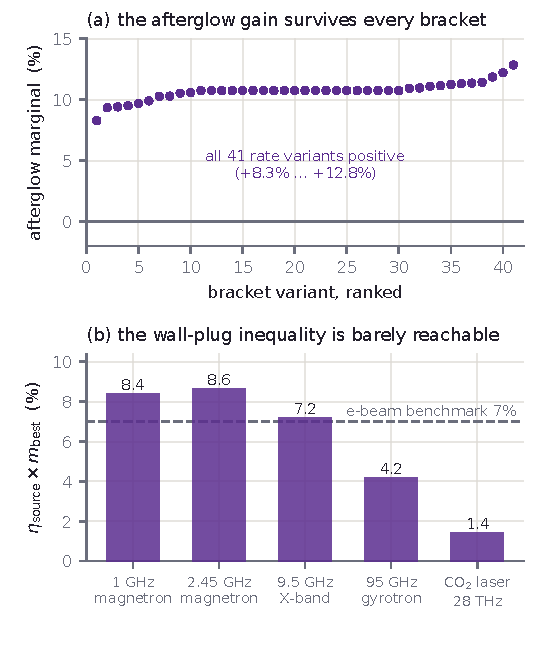
\includegraphics[width=\columnwidth]{fig_robust_and_wallplug.pdf}
\caption{\label{fig:robust}(a)~The one laser-positive afterglow case
(Ne-optimized cell) under all 41 rate-bracket and literature-conflict
variants: every variant stays positive ($+8.3\%$ to $+12.9\%$). (b)~The
wall-plug inequality: source efficiency times the best (and fragile)
marginal, by band, against the ${\approx}7\%$ e-beam benchmark. Data:
recorded run artifacts; figures regenerated by the included script.}
\end{figure}

\begin{figure}[t]
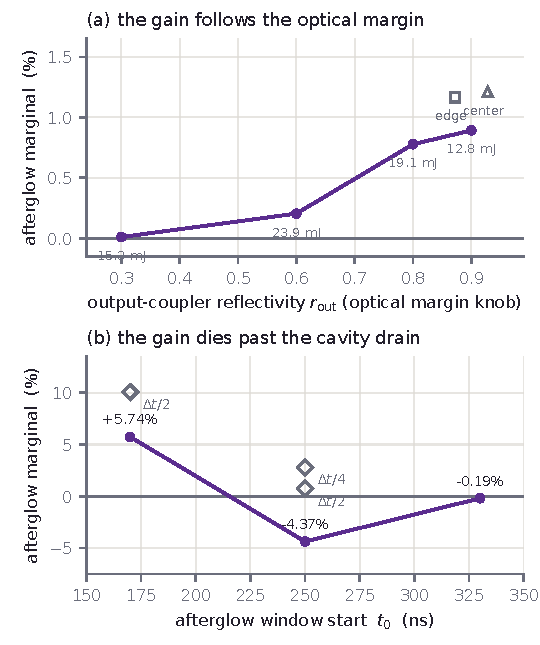
\includegraphics[width=\columnwidth]{fig_1d_verification.pdf}
\caption{\label{fig:oned}One-dimensional verification of the
late-extraction mechanism (independent discharge model, afterglow
window, absorbed power fixed at 250~kW). (a)~Marginal versus
output-coupler reflectivity (300-ns horizon); the annotated baseline
outputs are non-monotone while the marginal is monotone --- it tracks
photon lifetime, not laser performance. Open markers: edge- and
center-weighted deposition variants at $r_{\rm out}=0.9$.
(b)~Marginal versus window start at the high-margin point (500-ns
horizon, full drain captured); open diamonds are timestep-refined
repeats ($\Delta t/2$, $\Delta t/4$).}
\end{figure}

\subsection{Why it is very difficult}
\label{sec:difficult}

Five quantitative walls separate ``real'' from ``useful.''

\emph{(1) The efficiency ceiling at feasible coupling.} Across all
eight benchmarks and both tiers, no blended efficiency moves by more
than $0.0056$~percentage points (kinetic tier: $0.0036$). The positive
marginal must exceed the cell's own efficiency for the microwave joules
in the denominator to pay; even the $+10\%$ marginal of
Sec.~\ref{sec:real} barely clears its cell's $6.19\%$, and the co-pump
marginals that exceed their cells' $\eta_0$ do so by amounts worth
${\lesssim}0.003$~pp at the stated coupling.

\emph{(2) The conductivity pinning.} Prescribing more afterglow power
does not reach the reduced fields where electron-impact formation
pays ($E/N\gtrsim20$--30~Td): the conductive plasma settles at
${\lesssim}2$~Td at any injected power (probed to 1~GW), because added
power raises $n_e$ faster than $E$. The one heat-positive route
(direct excitation, whose rate rises by eight orders of magnitude from
0.5~eV to the 30-Td swarm point) is therefore unreachable in the
afterglow.

\emph{(3) The supply-chain inversion.} As measured by the audit above,
both feedstocks of excimer formation fall when the electrons are
heated; the identical audit of the ArF chain (six direct formation
rows, all heavy-particle) returns the same verdict with slightly worse
positioning. Electron heating pays in laser families whose upper level
is pumped by electron impact at eV energies (CO$_2$/CO class); the
excimer chain is the wrong class.

\emph{(4) The wall-plug inequality and the frequency question.} With
collision rates $\nu_m=0.9$--$8.9\times10^{12}\,$s$^{-1}$ over the
operating band, the collisional/field-oscillation crossover sits near
0.3~THz: below it the plasma cannot distinguish 1~GHz from 300~GHz
(equal absorption lengths, 1.8--2.0~mm at beam-on electron density),
and above it coupling collapses as $\omega^{-2}$. Wall-plug viability
requires $\eta_{\rm source}\times m > \eta_{\rm beam}\approx7\%$:
Fig.~\ref{fig:robust}(b) shows only magnetron-class sources times the
\emph{most favorable and least robust} marginal ($+12.5\%$) barely
clear it (8.4--8.6\%); millimeter-wave gyrotrons (4.2\%) and CO$_2$
lasers (1.4\%) do not. The same 2-mm absorption length implies the
deposition is a moving skin in any cell larger than centimeters ---
the uniform-coupling assumption of every model here is an upper bound
that real launch geometry can only degrade.

\emph{(5) The during-pulse sign is one uncertain rate wide.} The
co-pump marginal at the high-power cell's plateau is $+8.0\%$
nominally, and \emph{every} bracket variant but one leaves it positive.
The exception owns the sign: stepwise ionization of the krypton
metastable, $e+\mathrm{Kr}^*\!\to\mathrm{Kr}^++2e$. Mapping the
marginal against that single multiplier [Fig.~\ref{fig:during}(a)]
gives a sign-positive window of $\times0.49$--$\times1.99$ about the
nominal rate --- geometrically centered on it, with two zero
crossings inside the $\times3$ uncertainty band appropriate to the
rate's estimated provenance. The sign is therefore \emph{undecidable at
current rate knowledge, and decidable by a factor-two determination of
one rate}. Consistently, the independent kinetic tier (a different
effective rate set) returns $-2.7\%$ to $-4.5\%$ at the same nominal
point, and the independent 1-D model's co-pump marginal collapses from
$+16.6\%$ at 50~ps to $-24.8\%$ and $-5.8\%$ at 25 and 12.5~ps
[Fig.~\ref{fig:during}(b)]: the coarse-timestep positive is a
discretization artifact, and the fine-timestep values are small and
negative while the baseline is still converging.

\begin{figure}[t]
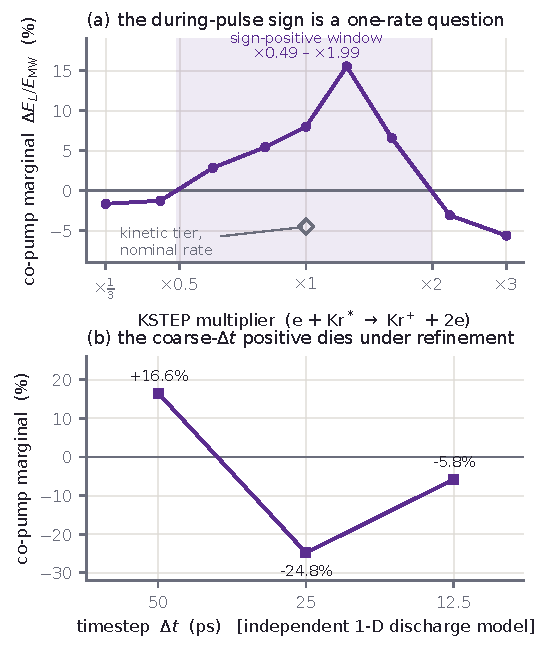
\includegraphics[width=\columnwidth]{fig_during_pulse.pdf}
\caption{\label{fig:during}(a)~Co-pump marginal at the high-power
cell's lasing plateau versus the multiplier on the one sign-controlling
rate ($e+\mathrm{Kr}^*\!\to\mathrm{Kr}^++2e$), swarm tier. The sign is
positive only inside $\times0.49$--$\times1.99$ (shaded); the open
diamond is the independent kinetic tier at the nominal rate. (b)~The
independent 1-D discharge model's co-pump marginal under timestep
refinement.}
\end{figure}

\section{Discussion}

\emph{What the study licenses an experimentalist to claim.} A
microwave window \emph{will} produce a measurable, model-robust
fluorescence response in essentially any e-beam-pumped configuration
--- reheating is feasible as an observable and as plasma physics. A
laser-energy gain from afterglow reheating exists in a specific,
predictable regime --- a cavity still extracting through the window
--- at the $+10\%$-per-microwave-joule level, and our bracket analysis
says a failure to observe it there would falsify the model rather than
the instrument. What no configuration supports is a material
improvement of blended efficiency at feasible coupling: the levers
that actually move these devices are conventional (halogen fraction,
pressure, optics, buffer choice --- a measured ladder from 1.54\% to
6.19\% in this engine, roughly $10^3$ times any electromagnetic
effect found here).

\emph{What would decide the open questions.} (i)~A factor-two
determination of the Kr$^*$ stepwise-ionization rate --- by literature
adjudication of the metastable ionization cross section, by a driven
relaxation measurement in the PIC code, or by experiment --- decides
the during-pulse sign within the swarm framework.
(ii)~Completion of the kinetic-tier run of the Ne-optimized afterglow
case decides whether the one robust positive is also tier-stable in
the same cell. (iii)~On the bench, gain-referenced twin shots (window
on/off at fixed fill) in a high-margin cell, with the absorbed
microwave energy closed by a full-wave deposition map rather than by
forward power, measure the marginal directly, and scanning the window
delay traces the drain curve of Fig.~\ref{fig:oned}(b) --- the
mechanism's most direct experimental signature; shot counts for stated
significance levels follow from the twin-difference variances measured
here.

\emph{Limitations.} The 0-D engine cannot express transverse structure
(filamentation and arc instability are the historical failure mode of
during-discharge heating, and are invisible here); the 1-D model
resolves the gap direction only, though it suffices to verify the
channel's margin, timing, and deposition-locality behavior
(Sec.~\ref{sec:real}). Both microwave treatments prescribe the
absorbed power; the 1-D profile ladder bounds the deposition-locality
error (second-order), but launch-geometry effects proper ---
reflection, standing waves, the measured 2-mm skin against a real
vessel --- remain outside both models. The reduced kinetics sets, while
literature-anchored, carry the bracket uncertainties used above by
construction. All results are predictions; no reheat experiment has
yet been scored against them.

\section{Conclusion}

In silico, microwave reheating of e-beam-pumped excimer plasmas is
(i)~a robust, cross-model observable through gain-proportional
fluorescence; (ii)~genuinely laser-positive in one narrow,
mechanistically understood regime --- late extraction from a
high-margin cavity --- with a sign that survives every rate bracket,
solver, and model-family perturbation applied; and (iii)~very
difficult to convert into device efficiency: blended gains are capped
at the $10^{-3}$-percentage-point scale at realistic coupling, the
afterglow plasma self-limits the attainable field, the excimer supply
chemistry weakens under electron heating, the wall-plug inequality is
at best marginal, and the one potentially larger channel (during-pulse
co-pumping) has a sign that current rate knowledge cannot fix. The
constructive outputs are precise: one rate to measure to a factor of
two, one regime in which to run twin-shot tests, and one observable
--- fluorescence --- whose positive response must not be mistaken for
efficiency.

\begin{acknowledgments}
\todo{Insert program-approved funding and collaboration acknowledgments
verbatim; do not paraphrase. Acknowledge the author of the independent
1-D discharge model by name with permission.}
\end{acknowledgments}

\section*{Data availability}

All twin-pair results, bracket tables, the rate-multiplier map, and
the frequency scan are recorded as JSON artifacts alongside the
engines' changelogs in the project workspace; the figures in this
draft are regenerated from those artifacts by the included script
(\texttt{make\_figs.py}). \todo{public archive/DOI before submission}

\begin{thebibliography}{9}
\bibitem{electra} \todo{Electra KrF/ArF program reference (NRL);
e.g.\ Wolford et al., and the recorded ArF peak-efficiency point used
as the anchor.}
\bibitem{hybridconcept} \todo{hybrid e-beam + microwave pumping
concept reference, or drop the sentence.}
\bibitem{loki} \todo{LoKI-MC citation: Tejero-del-Caz et al., Plasma
Sources Sci.\ Technol.\ (LisbOn KInetics); verify which of LoKI-B /
LoKI-MC papers applies.}
\bibitem{oned} \todo{the independent 1-D KrF discharge fluid model ---
cite the author's code/paper with permission.}
\bibitem{kannari} \todo{Kannari et al.\ KrF kinetics benchmark (1985)
used as the anchor cell.}
\end{thebibliography}

\end{document}
